
%(BEGIN_QUESTION)
% Copyright 2008, Tony R. Kuphaldt, released under the Creative Commons Attribution License (v 1.0)
% This means you may do almost anything with this work of mine, so long as you give me proper credit

Hvis et sett med seks elektromagnetspoler plasseres rundt periferien av en sirkel og mates med trefase AC, og et magnetkompass plasseres i sentrum av sirkelen, vil kompassnålen rotere fordi den påvirkes av et roterende magnetfelt produsert av spolene:

$$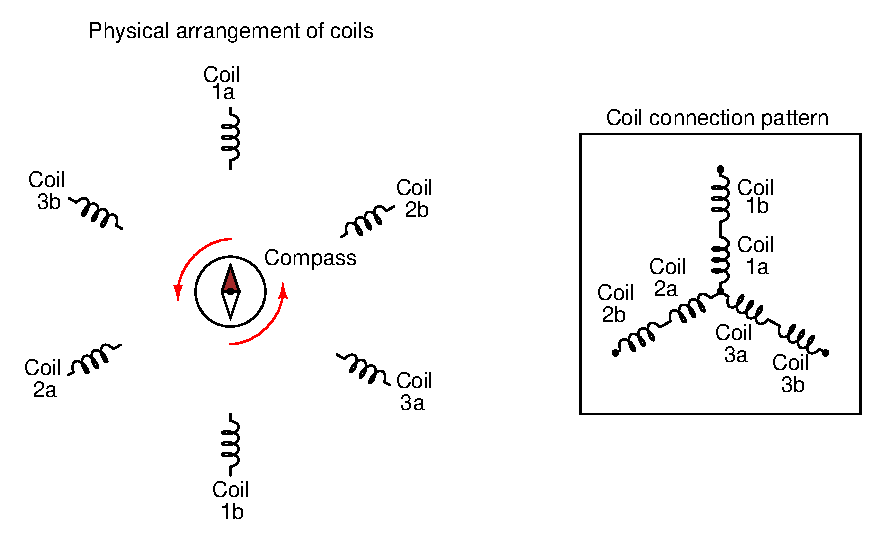
\includegraphics[width=15.5cm]{i01443x01.eps}$$

Forklar hvorfor magnetfeltet fra statorspolene ser ut til å rotere, og beregn også rotasjonshastigheten til dette feltet dersom trefase AC-frekvensen er 60 Hz. Basert på rotasjonen som er vist (pilene), hva er {\it faserekkefølgen} til AC-forsyningen til motoren?

\vskip 10pt

Bestem også hva som måtte endres i dette scenariet for at kompassnålen skal rotere med bare {\it halvparten} av nåværende hastighet.

\vskip 10pt

Bestem også hva som måtte endres i dette scenariet for at kompassnålen skal rotere i {\it motsatt retning} av nå.

\vskip 20pt \vbox{\hrule \hbox{\strut \vrule{} {\bf Forslag til sokratisk diskusjon} \vrule} \hrule}

\begin{itemize}
\item{} Hvorfor bygges spolene i en virkelig trefasemotor i par, slik som vist her? Hvorfor ikke bare ha tre spoler i stedet for seks?
\item{} Anta at én av linjene i trefaseforsyningen til denne motoren blir brutt, slik at strøm hindres gjennom ett av spoletsettene i statoren. Vil kompassnålen fortsatt rotere? Hvorfor eller hvorfor ikke?
\item{} Hvordan ville statorspole-arrangementet sett ut for en {\it fire}fase elektrisk motor?
\end{itemize}

\underbar{file i01443}
%(END_QUESTION)





%(BEGIN_ANSWER)

Det er nyttig å huske hvordan trefaseeffekt {\it genereres} når man skal svare på dette spørsmålet: Vi genererer trefaseeffekt ved å rotere en magnet i sentrum av tre spoletsett, plassert 120$^{o}$ fra hverandre rundt sirkelen.

\vskip 10pt

Magnetfeltet ser ut til å rotere fordi statorviklingene blir spenningssatt forskjøvet i en 1-2-3-sekvens. Dette ligner en rekke blinkende ``julelys'' som ser ut til å bevege seg fordi lysene blinker i en sekvens med tydelig retning.

\vskip 10pt

Kompassnålens rotasjonshastighet blir 3600 RPM (60 omdreininger per sekund) ved forsyningsfrekvens 60 Hz. For å halvere denne hastigheten må vi enten legge til dobbelt så mange poler i motoren, eller halvere frekvensen (30 Hz).

\vskip 10pt

For å reversere retningen på nålen må faserekkefølgen på forsyningen byttes. Dette kan gjøres ved å bytte om på hvilke som helst to av de tre kraftlederne til statoren.

%(END_ANSWER)





%(BEGIN_NOTES)


%INDEX% Final Control Elements, motor: rotating magnetic field

%(END_NOTES)

